\documentclass[a4paper,12pt]{report}

%Русский язык
\usepackage[T2A]{fontenc}
\usepackage[utf8]{inputenc}
\usepackage[english,russian]{babel}
\usepackage{cmap}

%Работа с кодом
\usepackage{listings}
\usepackage{color}

\definecolor{green}{rgb}{0,0.6,0}
\definecolor{gray}{rgb}{0.5,0.5,0.5}
\definecolor{red}{rgb}{0.6,0,0}

\lstset{
        language=Python, 
        basicstyle=\small\ttfamily, 
        numberstyle=\tiny,           
        columns=flexible,
        stepnumber=1,                   
        numbersep=5pt,        
        showspaces=false,
        showstringspaces=false,
        showtabs=false,
        tabsize=2,                
        captionpos=b,              
        breaklines=true,           
        breakatwhitespace=false,
        keywordstyle=\color{green},
        commentstyle=\color{gray},
        stringstyle=\color{red},      
}

%Математика
\usepackage{amsmath,amsfonts,amssymb,amsthm,mathtools} 

%Изображения
\usepackage{float}
\usepackage{graphicx}
\graphicspath{ {./img/} }

%Поля страницы
\usepackage{geometry} 
\geometry{left=2.3cm} 
\geometry{right=1.8cm} 
\geometry{top=2cm} 
\geometry{bottom=2.5cm} 

%Отступы
\usepackage{indentfirst}
\setlength{\parskip}{0cm}

\begin{document} 

\begin{titlepage}
\newpage
	\begin{center}
		\large Санкт-Петербургский политехнический университет Петра Великого\\
		Институт компьютерных наук и технологий\\
		Высшая школа интеллектуальных систем и суперкомпьютерных технологий\\
	\end{center}
\vspace{7cm}

\begin{center}
		\large \textbf{Отчёт по лабораторной работе №9} \\
		\textbf{Дисциплина:} Телекоммуникационные технологии\\
		\textbf{Тема:} Дифференцирование и интегрирование
\end{center}
\vspace{4cm}
	
\begin{flushright}
		\large Работу выполнил:\\ Ляшенко В.В.\\
		Группа: 3530901/80201\\
		Преподаватель:\\ Богач Н.В.
\end{flushright}

\vspace{\fill}
\begin{center}
	\large Санкт-Петербург\\ 2021
	\end{center}
\end{titlepage}

\tableofcontents
\listoffigures
\lstlistoflistings

\chapter{Упражнение 9.1}
    В начале мы запустим примеры из \texttt{chap09.ipynb}.
    
    В пособии сказано, что некоторые примеры не работают с апериодическими сигналами. Заменим периодический пилообразный сигнал на непериодические данные Facebook и посмотрим, что случится.
    
    Сначала создадим сигнал (Рис.1.1).
\begin{lstlisting}[caption=Создание сигнала Facebook]
       import pandas as pd
       from thinkdsp import Wave

       df = pd.read_csv('FB_2.csv', header=0, parse_dates=[0])
       ys = df['Close']
       in_wave = Wave(ys, framerate=1)
       in_wave.plot()
       decorate(xlabel='Time (days)', ylabel='Price ($)')
\end{lstlisting}
\begin{figure}[H]
        \centering
        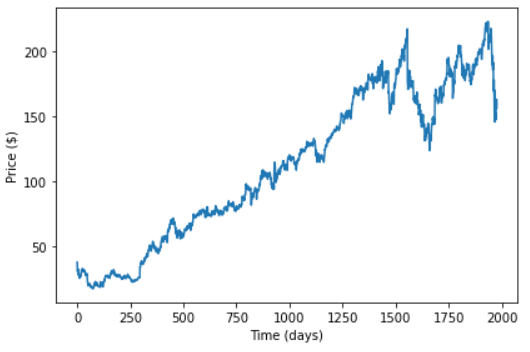
\includegraphics[width=0.8\textwidth]{fig1-1.PNG}
        \caption{Сигнал Facebook}
        \label{fig:fig1-1}
\end{figure} 

    Построим его спектр (Рис.1.2).    
\begin{lstlisting}[caption=Построение спектра Facebook]
       in_spectrum = in_wave.make_spectrum()
       in_spectrum.plot()
       decorate(xlabel='Frequency (Hz)', ylabel='Amplitude')
\end{lstlisting}
\begin{figure}[H]
        \centering
        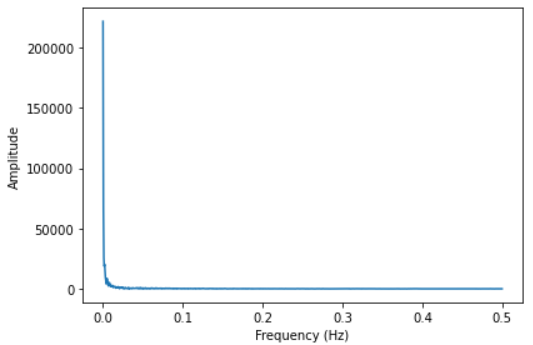
\includegraphics[width=0.8\textwidth]{fig1-2.PNG}
        \caption{Спектр Facebook}
        \label{fig:fig1-2}
\end{figure} 

    Теперь получим выходной сигнал, который является совокупной суммой входных сигналов (Рис.1.3), и его спектр (Рис.1.4).  
\begin{figure}[H]
        \centering
        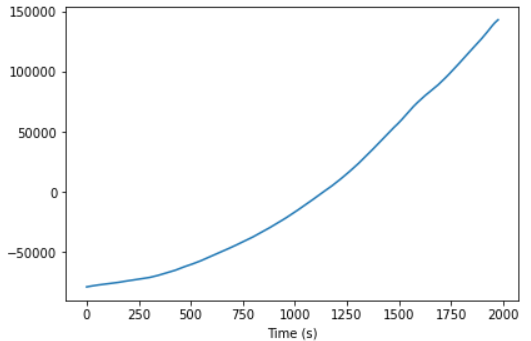
\includegraphics[width=0.8\textwidth]{fig1-3.PNG}
        \caption{Выходной сигнал}
        \label{fig:fig1-3}
\end{figure}   
\begin{figure}[H]
        \centering
        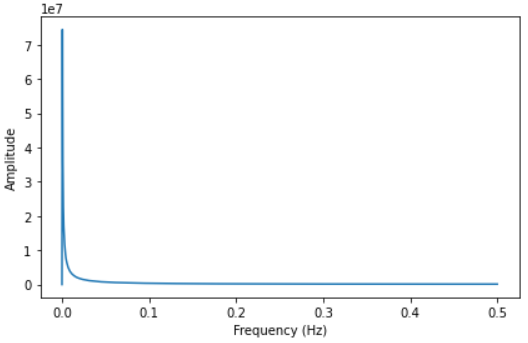
\includegraphics[width=0.8\textwidth]{fig1-4.PNG}
        \caption{Спектр выходного сигнала}
        \label{fig:fig1-4}
\end{figure} 

    Теперь посмотрим на отношение между входными и выходными данными (Рис.1.5).
\begin{figure}[H]
        \centering
        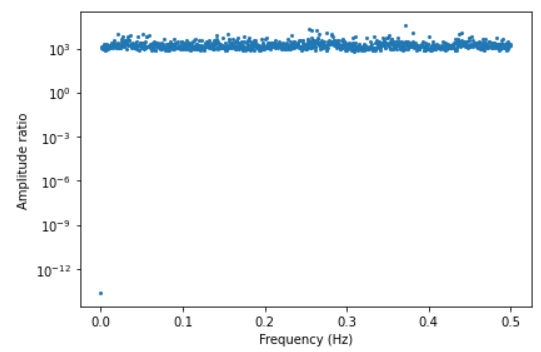
\includegraphics[width=0.8\textwidth]{fig1-5.PNG}
        \caption{Отношение входных и выходных данных}
        \label{fig:fig1-5}
\end{figure} 

    Построим фильтр для нарастающей суммы и сравним его с фильром интегрирования.
\begin{figure}[H]
        \centering
        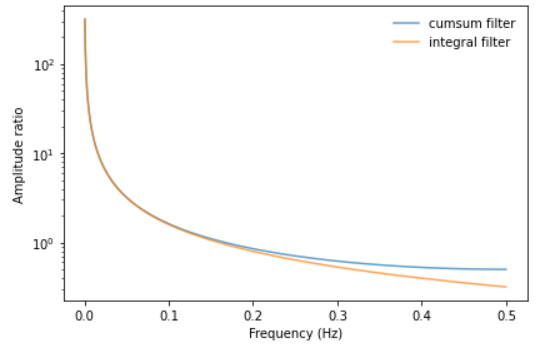
\includegraphics[width=0.8\textwidth]{fig1-6.PNG}
        \caption{Фильтры нарастающей суммы и интегрирования}
        \label{fig:fig1-6}
\end{figure}  
    
    Как мы видим на рис.1.6, графики сначала полностью совпадают, а под конец немного расходятся.
    
    Затем мы можем сравнить вычисленное отношение с фильтром. 
\begin{figure}[H]
        \centering
        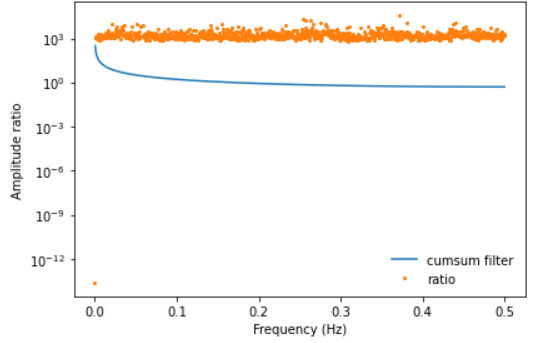
\includegraphics[width=0.8\textwidth]{fig1-7.PNG}
        \caption{Сравнение отношения и фильтра}
        \label{fig:fig1-7}
\end{figure}   

    Здесь случается первое расхождение (Рис.1.7). Данные графики должны совпадать. Это означало бы что фильтр \texttt{cumsum} является обратным фильтру \texttt{diff}. Но этого не происходит.
    
    Теперь применим фильтр \texttt{cumsum} в частотной области.
\begin{figure}[H]
        \centering
        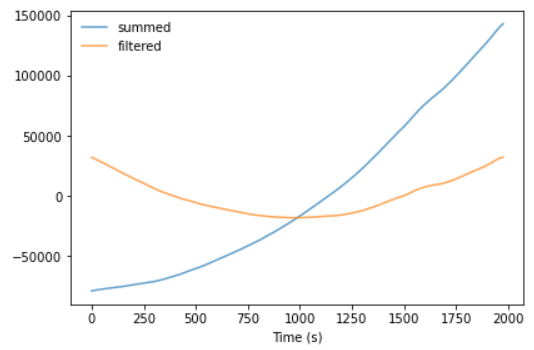
\includegraphics[width=0.8\textwidth]{fig1-8.PNG}
        \caption{Сравнение суммирования и фильтрации}
        \label{fig:fig1-8}
\end{figure} 

    На рис.1.8 вновь видим пример неправильной работы. Графики не совпадают.
         
\chapter{Упражнение 9.2}
    В этом упражнении изучается влияние \texttt{diff} и \texttt{differentiate} на сигнал.
    
    Создадим треугольный сигнал и напечатаем его (Рис.2.1). 
\begin{lstlisting}[caption=Создание треугольного сигнала]
       from thinkdsp import TriangleSignal

       triangle = TriangleSignal(freq=50).make_wave(duration=0.1, framerate=44100)
       triangle.plot()
       decorate(xlabel='Time (s)')
\end{lstlisting}
\begin{figure}[H]
        \centering
        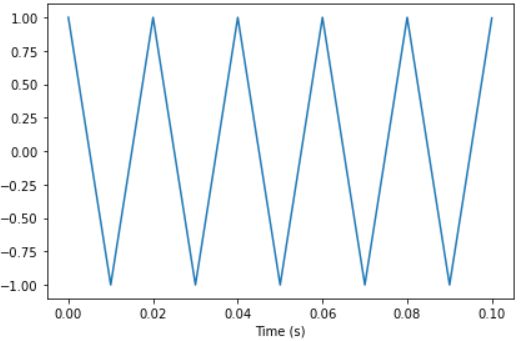
\includegraphics[width=0.8\textwidth]{fig2-1.PNG}
        \caption{Треугольный сигнал}
        \label{fig:fig2-1}
\end{figure} 

    Применим к нему \texttt{diff} и напечатаем результат (Рис.2.2).
\begin{lstlisting}[caption=Использование diff]
       out_wave = triangle.diff()
       out_wave.plot()
       decorate(xlabel='Time (s)')
\end{lstlisting}
\begin{figure}[H]
        \centering
        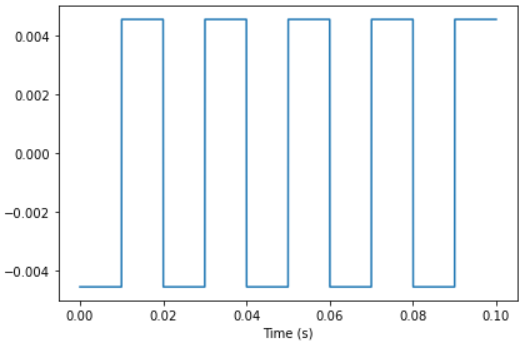
\includegraphics[width=0.8\textwidth]{fig2-2.PNG}
        \caption{Результат diff}
        \label{fig:fig2-2}
\end{figure} 

   Вычислим спектр треугольного сигнала, применим к нему \texttt{differentiate} и напечатаем (Рис.2.3).
\begin{lstlisting}[caption=Использование differentiate]
       out_wave2 = triangle.make_spectrum().differentiate().make_wave()
       out_wave2.plot()
       decorate(xlabel='Frequency (Hz)')
\end{lstlisting}
\begin{figure}[H]
        \centering
        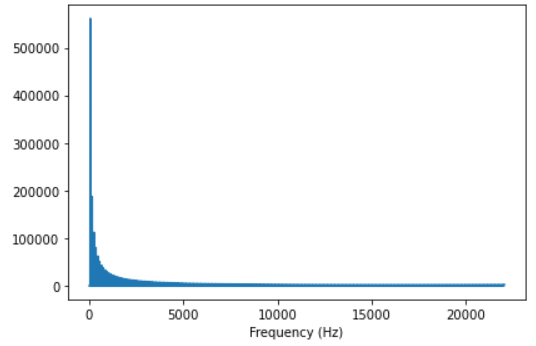
\includegraphics[width=0.8\textwidth]{fig2-3.PNG}
        \caption{Результат differentiate}
        \label{fig:fig2-3}
\end{figure}
    
    Теперь преобразуем спектр обратно в сигнал и напечатем его (Рис.2.4).
\begin{lstlisting}[caption=Преобразование спектра в сигнал]
       out_wave2.make_wave().plot()
       decorate(xlabel='Time (s)')
\end{lstlisting}
\begin{figure}[H]
        \centering
        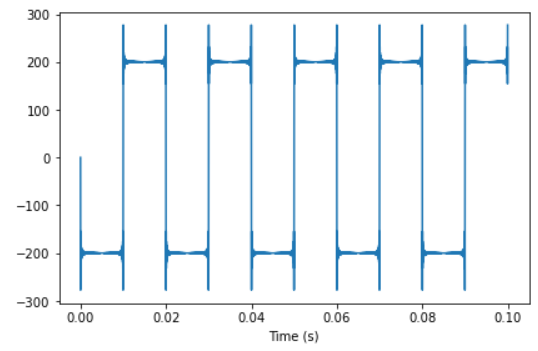
\includegraphics[width=0.8\textwidth]{fig2-4.PNG}
        \caption{Спектр в сигнал}
        \label{fig:fig2-4}
\end{figure}   
       
    Когда мы берём спектральную производную, мы получаем "звон" вокруг разрывов.
    
    С математической точки зрения это происходит, потому что производная треугольного сигнала не определена в вершинах треугольников.
    
\chapter{Упражнение 9.3}
    В данном упражнении изучается влияние \texttt{cumsum} и \texttt{integrate} на сигнал.
    
    Создадим прямоугольный сигнал и напечатаем его (Рис.3.1). 
\begin{lstlisting}[caption=Создание прямоугольного сигнала]
       from thinkdsp import SquareSignal

       square = SquareSignal(freq=50).make_wave(duration=0.1, framerate=44100)
       square.plot()
       decorate(xlabel='Time (s)')
\end{lstlisting}
\begin{figure}[H]
        \centering
        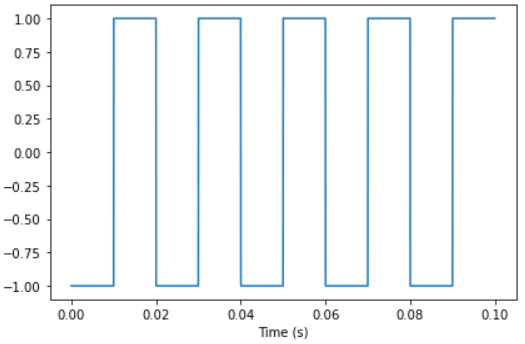
\includegraphics[width=0.8\textwidth]{fig3-1.PNG}
        \caption{Прямоугольный сигнал}
        \label{fig:fig3-1}
\end{figure} 

    Применим к нему \texttt{cumsum} и напечатаем результат (Рис.3.2).
\begin{lstlisting}[caption=Использование cumsum]
       out_wave = square.cumsum()
       out_wave.plot()
       decorate(xlabel='Time (s)')
\end{lstlisting}
\begin{figure}[H]
        \centering
        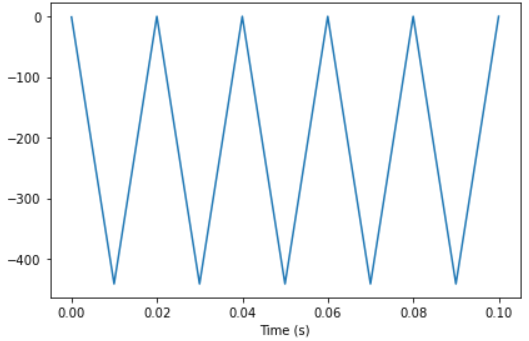
\includegraphics[width=0.8\textwidth]{fig3-2.PNG}
        \caption{Результат cumsum}
        \label{fig:fig3-2}
\end{figure} 

   Вычислим спектр прямоугольного сигнала, применим к нему \texttt{integrate} и напечатаем (Рис.3.3).
\begin{lstlisting}[caption=Использование integrate]
       spectrum = square.make_spectrum().integrate()
       spectrum.plot()
       decorate(xlabel='Frequency (Hz)')
\end{lstlisting}
\begin{figure}[H]
        \centering
        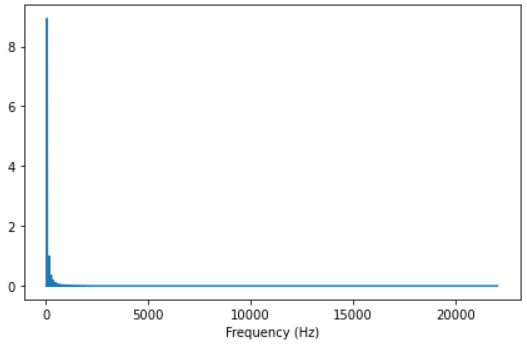
\includegraphics[width=0.8\textwidth]{fig3-3.PNG}
        \caption{Результат integrate}
        \label{fig:fig3-3}
\end{figure} 
    
    Теперь преобразуем спектр обратно в сигнал и напечатем его (Рис.3.4).
\begin{lstlisting}[caption=Преобразование спектра в сигнал]
       spectrum.hs[0] = 0
       out_wave2 = spectrum.make_wave()
       out_wave2.plot()
       decorate(xlabel='Time (s)')
\end{lstlisting}
\begin{figure}[H]
        \centering
        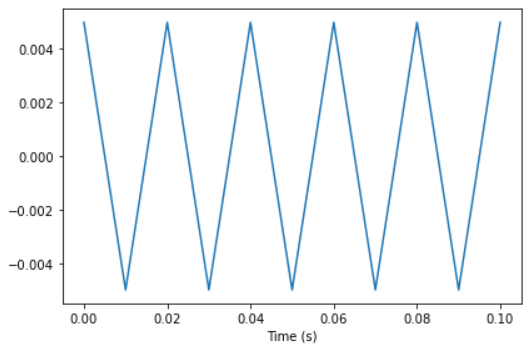
\includegraphics[width=0.8\textwidth]{fig3-4.PNG}
        \caption{Спектр в сигнал}
        \label{fig:fig3-4}
\end{figure}   

    Результаты \texttt{cumsum} и \texttt{integrate} с виду получились одинаковыми. Проверим, есть ли какие-то различия между этими функциями (Рис.3.5).
\begin{lstlisting}[caption=Сравнение cumsum и integrate]
       out_wave.unbias()
       out_wave.normalize()
       out_wave2.normalize()
       out_wave.plot()
       out_wave2.plot()
       decorate(xlabel='Time (s)')

       out_wave.max_diff(out_wave2)
\end{lstlisting}
\begin{figure}[H]
        \centering
        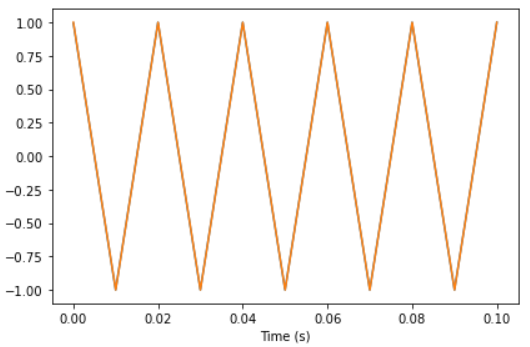
\includegraphics[width=0.8\textwidth]{fig3-5.PNG}
        \caption{Сравнение функций}
        \label{fig:fig3-5}
\end{figure} 

    Численно они тоже схожи, но с точностью около 3 цифр. 
      
\chapter{Упражнение 9.4}
    В этом упражнении изучается влияние двойного интегрирования.
            
    Создадим пилообразный сигнал, вычислим его спектр и дважды применим \texttt{integrate}. Затем напечатаем результирующий сигнал и его спектр.
\begin{lstlisting}[caption=Создание и работа с пилообразным сигналом]
       from thinkdsp import SawtoothSignal

       sawtooth = SawtoothSignal(freq=50).make_wave(duration=0.1, framerate=44100)
       spectrum = sawtooth.make_spectrum().integrate().integrate()
       spectrum.hs[0] = 0
       out_wave = spectrum.make_wave()
       out_wave.plot()
       decorate(xlabel='Time (s)')
\end{lstlisting}
\begin{figure}[H]
        \centering
        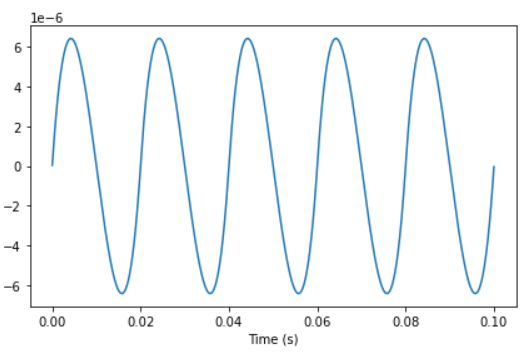
\includegraphics[width=0.8\textwidth]{fig4-1.PNG}
        \caption{Результирующий сигнал}
        \label{fig:fig4-1}
\end{figure}
\begin{lstlisting}[caption=Создание спектра результирующего сигнала]
       out_wave.make_spectrum().plot(high=500)
       decorate(xlabel='Frequency (Hz)')
\end{lstlisting} 
\begin{figure}[H]
        \centering
        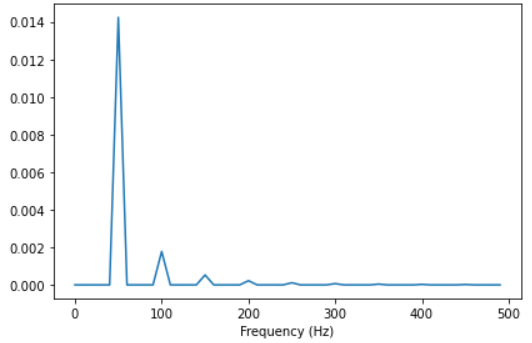
\includegraphics[width=0.8\textwidth]{fig4-2.PNG}
        \caption{Спектр результирующего сигнала}
        \label{fig:fig4-2}
\end{figure} 

    Из рис.4.1 мы можем видеть, что результат напоминает синусоиду. Причина в том, что интегрирование действует как фильтр нижних частот. Из спектра видно, что после двойного применения функции \texttt{integrate} мы отфильтровали почти все, кроме основных частот (Рис.4.2). 
    
\chapter{Упражнение 9.5}
    В данном упражнении изучается влияние второй разности и второй производной.
    
    Создадим \texttt{CubicSignal}, определённый в \texttt{thinkdsp}.
\begin{lstlisting}[caption=Создание кубического сигнала]
       from thinkdsp import CubicSignal

       cubic = CubicSignal(freq=0.0005).make_wave(duration=10000, framerate=1)
       cubic.plot()
\end{lstlisting}
\begin{figure}[H]
        \centering
        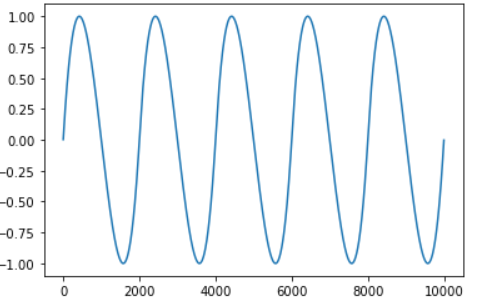
\includegraphics[width=0.8\textwidth]{fig5-1.PNG}
        \caption{Кубический сигнал}
        \label{fig:fig5-1}
\end{figure}     

    Вычислим его вторую разность, дважды применив \texttt{diff}. Напечатаем получившийся результат (Рис.5.2). 
\begin{lstlisting}[caption=Вычисление второй разности]
       out_wave = cubic.diff()
       out_wave = out_wave.diff()
       out_wave.plot()
       decorate(xlabel='Time (s)')
\end{lstlisting}
\begin{figure}[H]
        \centering
        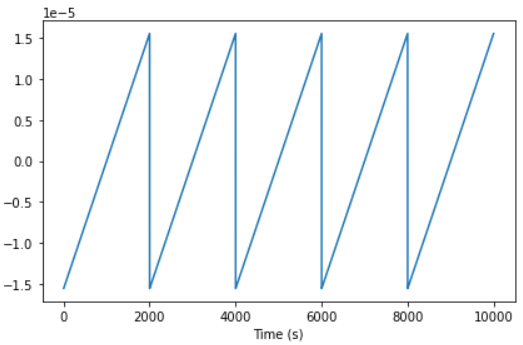
\includegraphics[width=0.8\textwidth]{fig5-2.PNG}
        \caption{Вторая разность кубического сигнала}
        \label{fig:fig5-2}
\end{figure} 
    
    Получившийся результат похож на пилообразный сигнал.
    
    Вычислим вторую производную, дважды применив \texttt{differentiate} к спектру. Напечатаем получившийся результат (Рис.5.3).
\begin{lstlisting}[caption=Вычисление второй производной]
       spectrum = cubic.make_spectrum().differentiate().differentiate()
       out_wave2 = spectrum.make_wave()
       out_wave2.plot()
       decorate(xlabel='Time (s)')
\end{lstlisting}
\begin{figure}[H]
        \centering
        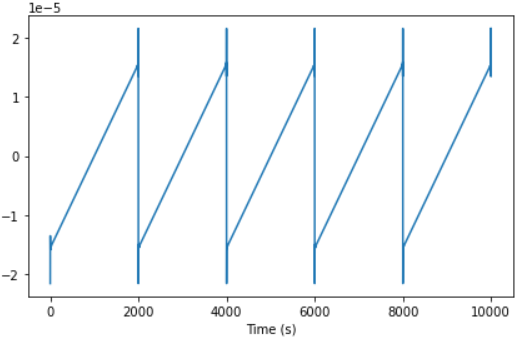
\includegraphics[width=0.8\textwidth]{fig5-3.PNG}
        \caption{Вторая производная кубического сигнала}
        \label{fig:fig5-3}
\end{figure} 

    Как видим, мы получили пилообразную форму с некоторым звоном.    
    
    Распечатаем фильтры, соответствующие второй разности и второй производной, и сравним их (Рис.5.4).
\begin{figure}[H]
        \centering
        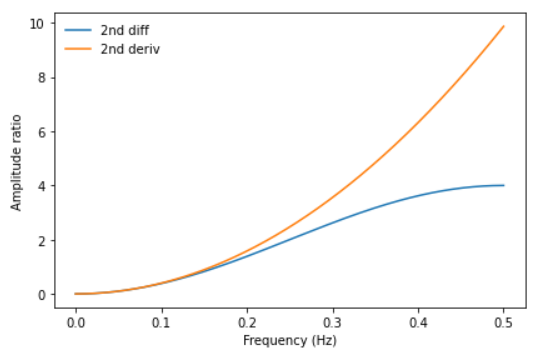
\includegraphics[width=0.8\textwidth]{fig5-4.PNG}
        \caption{Сравнение фильтров}
        \label{fig:fig5-4}
\end{figure} 

    Оба фильтра являются фильтрами высоких частот, которые усиливают компоненты самых высоких частот. Вторая производная параболическая, поэтому она сильнее всего усиливает самые высокие частоты. Вторая разность - хорошее приближение второй производной только на самых низких частотах, затем она существенно отклоняется.    

\chapter{Выводы}
    В результате выполнения данной работы мы изучили  функции дифференцирования и интегрирования, а также научились применять их на различных сигналах. 
\end{document}